\begin{frame}
\frametitle{More Detailed Example Applications}
\begin{itemize}
\item Flexible Flow-Shop with Transportation Times 
\begin{itemize}
\item J\&J, studies future factory design
\end{itemize}
\item Production Planning and Scheduling
\begin{itemize}
\item Multi-year capacity planning
\item For Siemens Energy, part of ASSISTANT project
\end{itemize}
\item Elevator Maintenance Planning and Scheduling
\begin{itemize}
\item Importance of decomposition
\item Combination with simulation
\end{itemize}
\item Selection of other problem types
\begin{itemize}
\item Only summary slides shown
\end{itemize}
\end{itemize}
\end{frame}


\mode<all>{\input{../summerschool2026/jj}}

\mode<all>{\input{../summerschool2026/siemensenergy}}

\mode<all>{\input{../summerschool2026/fieldservice}}

\section{Other Applications}

\begin{frame}
\frametitle{Other Noteworthy Applications}
\begin{itemize}
\item NVD LoadBuilder
\item Boliden Tara Mines Dewatering
\item Dental School Timetabling
\item Irish Naval Service Rostering
\item Data Centre Load Consolidation
\item Scheduling with Time Variable Energy Prices
\item Characterizing EDF Power Plants with Timeseries Constraints
\item Optical Network Design
\item Supplier Selection Problem
\item Optimizing UCC's CHP Plant Operation
\item CP Conference Paper Assignment Tool
\end{itemize}
\end{frame}

\begin{frame}
\frametitle{NVD LoadBuilder}
\begin{textblock*}{5cm}(9cm,-1cm)
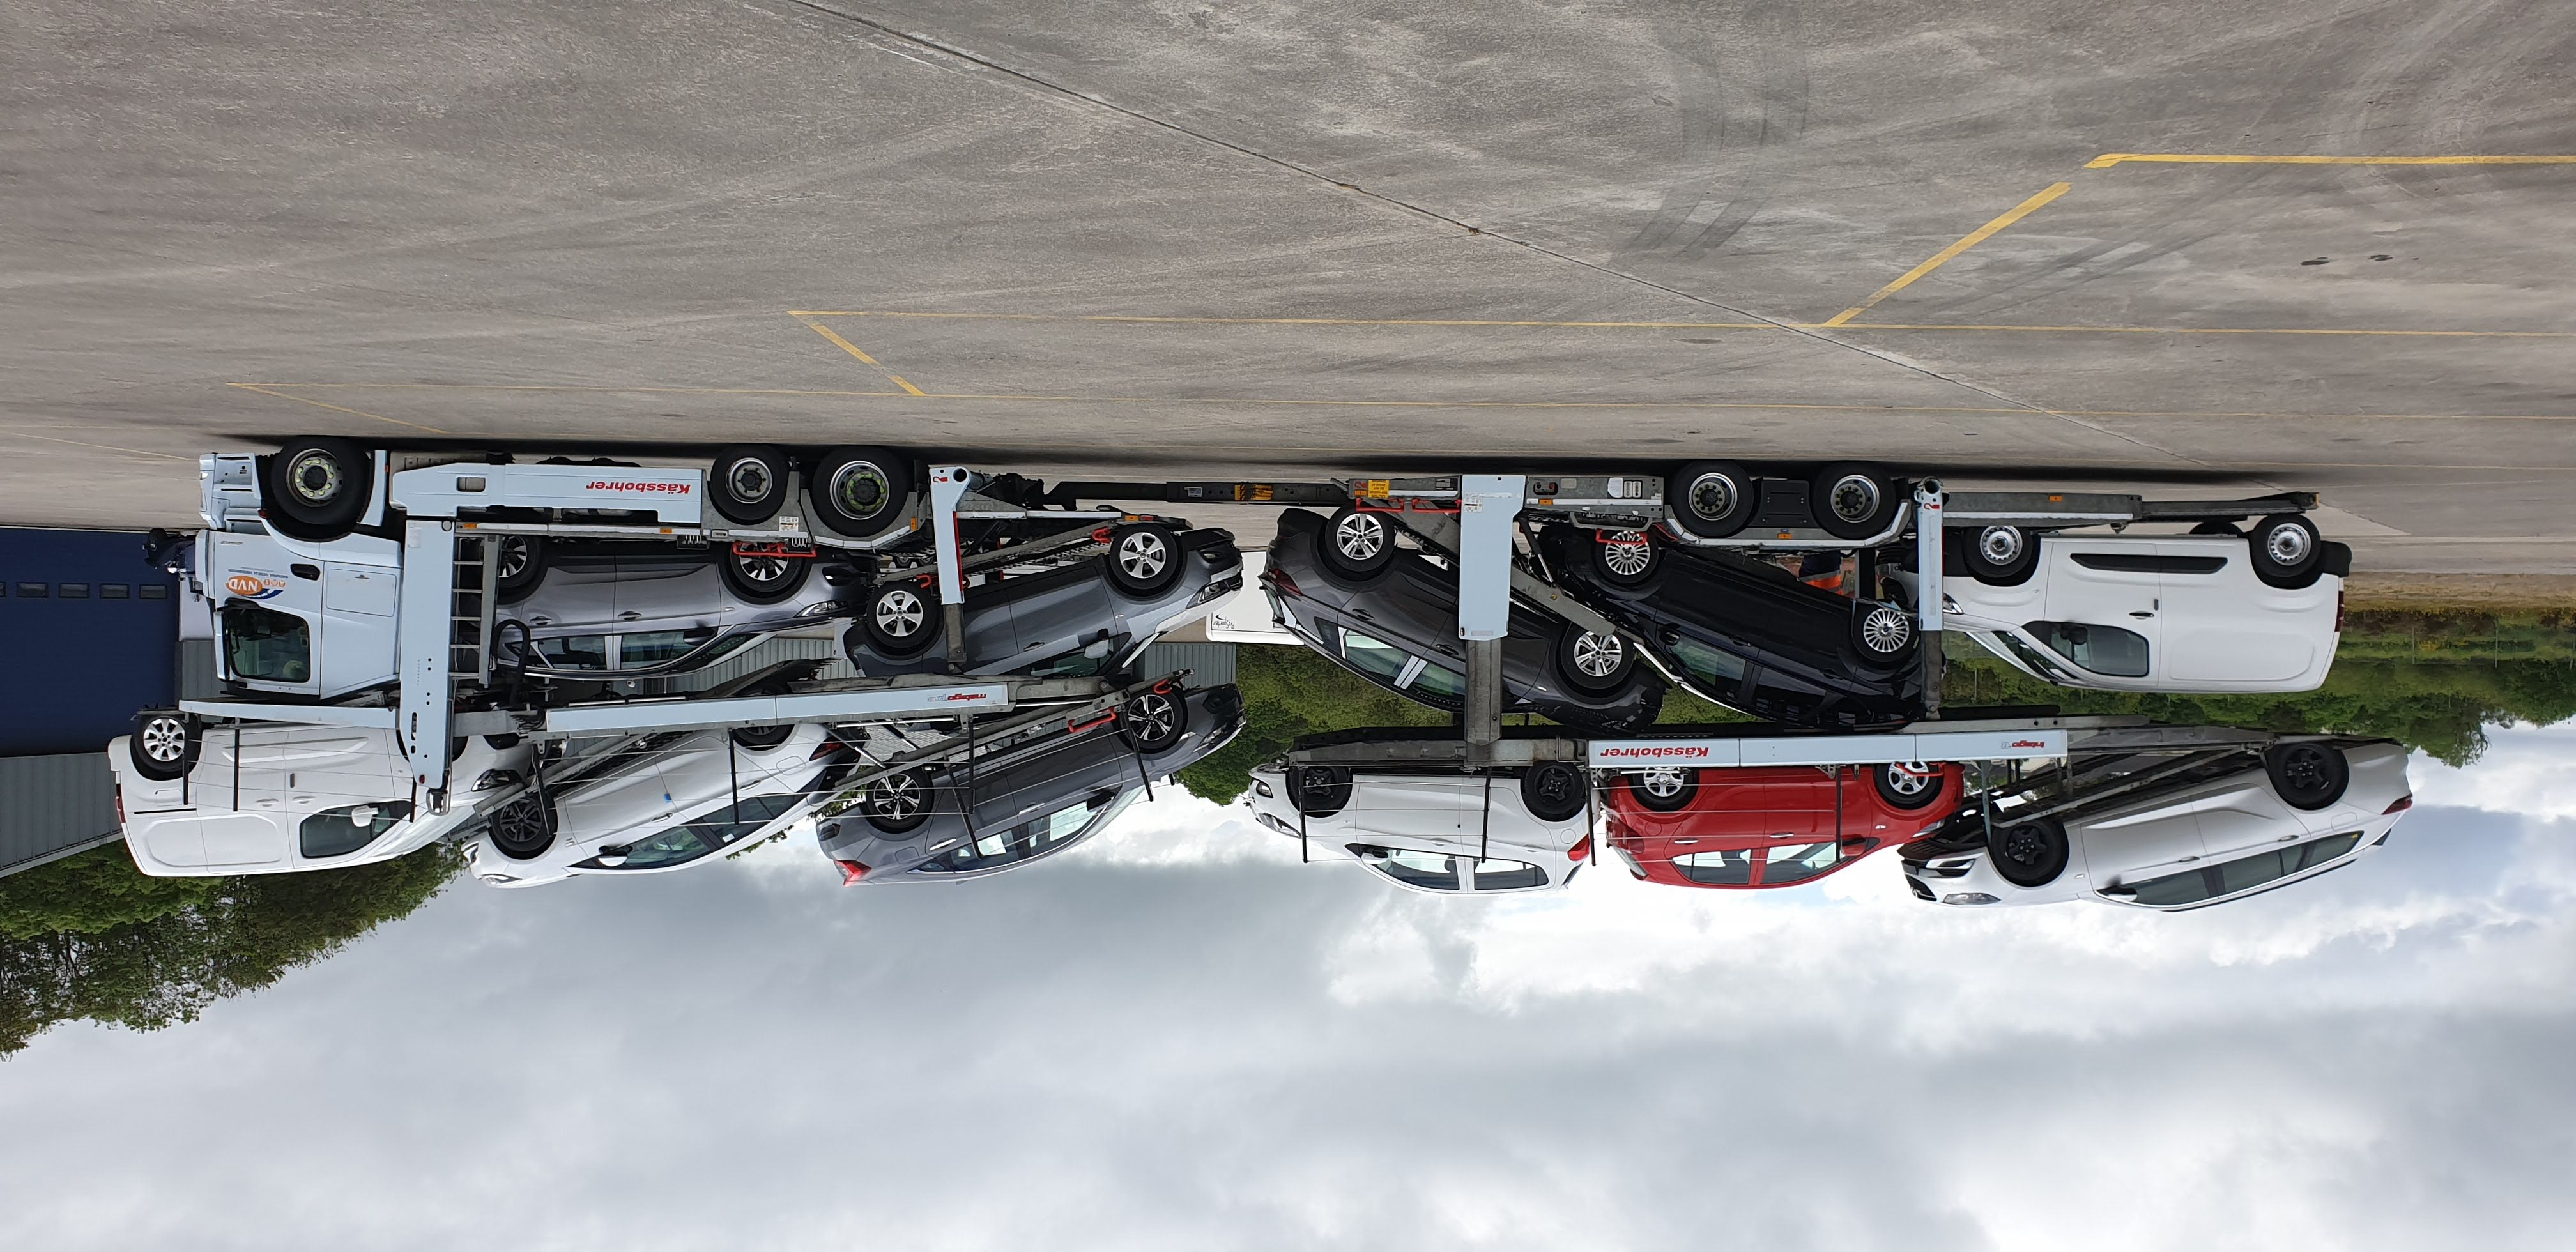
\includegraphics[width=5cm,angle=180]{images/metagointago}
\end{textblock*}

\begin{columns}[b]
\begin{column}{0.5\textwidth}
\begin{itemize}
\item Real-World Problem
\begin{itemize}
\item Deliver cars/vans from factory/ports to dealers
\item Group cars into loads for joint delivery
\item Using specialized transporters with complex configurations
\item Balance distance travelled, utilization of fleet, priority of orders
\end{itemize}
\item Status
\begin{itemize}
\item Operational at customer starting in 2020
\item Start-up company CMC to further develop tool
\end{itemize}
\end{itemize}
\end{column}
\begin{column}{0.5\textwidth}
\begin{itemize}
\item Research Challenges
\begin{itemize}
\item Vehicle routing problem with complex capacity constraints
\item Decide which cars to deliver today
\item What impact does this have tomorrow
\item Explaining solutions to end-user
\end{itemize}
\item Solution Approach
\begin{itemize}
\item Decomposition
\item MIP, Constraint Programming, Local Search, Data Analytics
\end{itemize}
\end{itemize}
\end{column}
\end{columns}
\end{frame}

\begin{frame}
\frametitle{Boliden Tara Mines Dewatering}
\begin{textblock*}{4cm}(9cm,-1cm)
%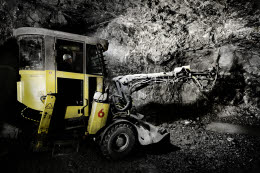
\includegraphics[width=4cm]{images/bolidentara}
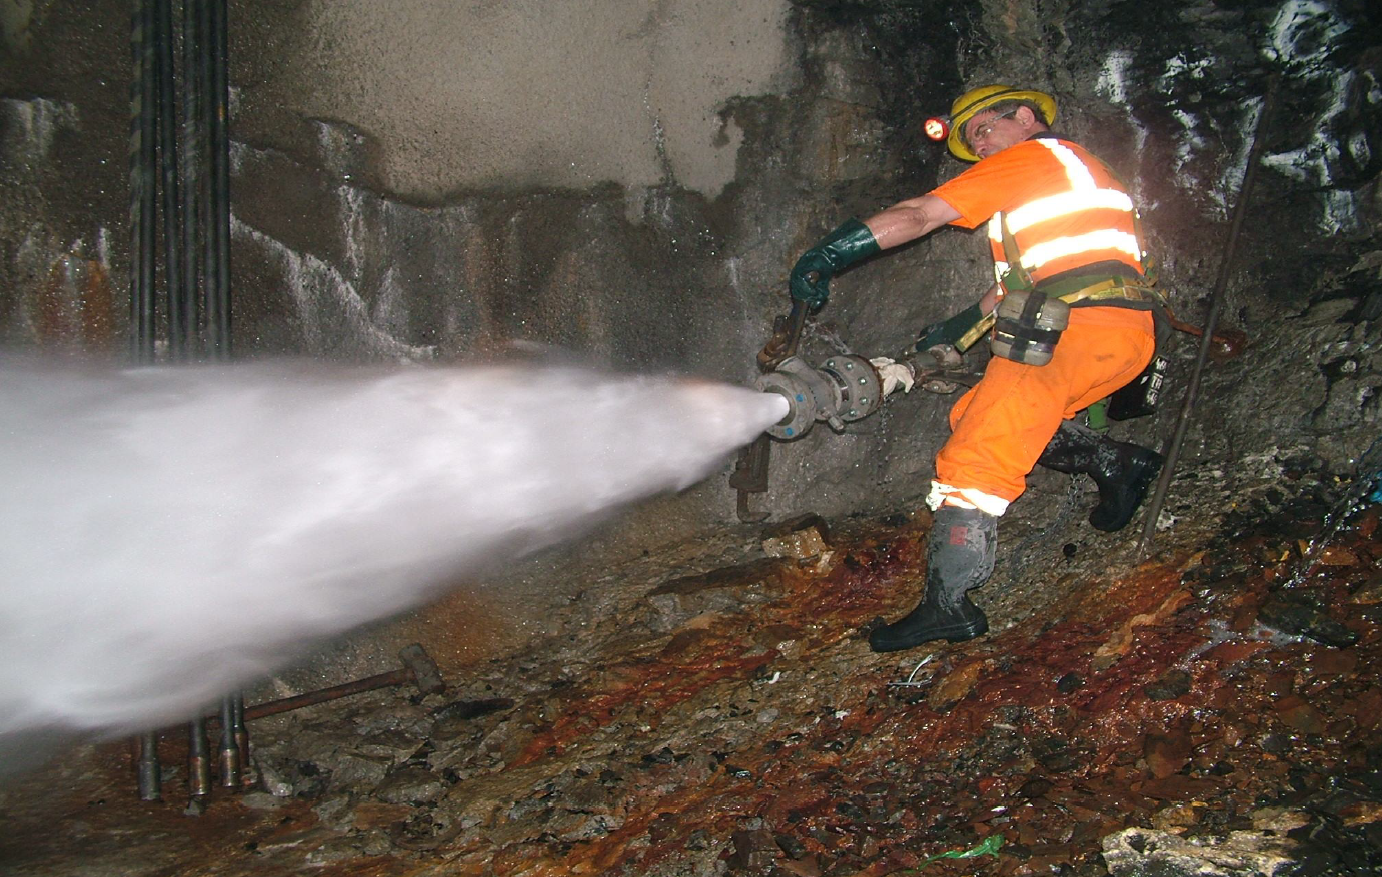
\includegraphics[width=4cm]{images/waterflow}
\end{textblock*}
\vspace{2cm}
\begin{columns}[b]
\begin{column}{0.5\textwidth}
\begin{itemize}
\item Real-World Problem
\begin{itemize}
\item When/how to pump water out of mine
\item Multiple pumps, reservoirs
\item Electricity cost major cost factor
\item Safe operation of mine paramount
\end{itemize}
\item Status
\begin{itemize}
\item Student-led project with DCU
\item Paper at AAAI 2016
\item Major flooding event in 2021
\end{itemize}
\end{itemize}
\end{column}
\begin{column}{0.5\textwidth}
\begin{itemize}
\item Research Challenges
\begin{itemize}
\item Scheduling with uncertain energy prices (real-time tariff)
\item Uncertain water ingress depends on operations
\item Capacity (min/max) constraints for storage 
\end{itemize}
\item Solution Approach
\begin{itemize}
\item Electricity price prediction
\item Optimization
\end{itemize}
\end{itemize}
\end{column}
\end{columns}
\end{frame}

\begin{frame}
\frametitle{Dental School Timetabling}
\begin{textblock*}{6cm}(8cm,-1cm)
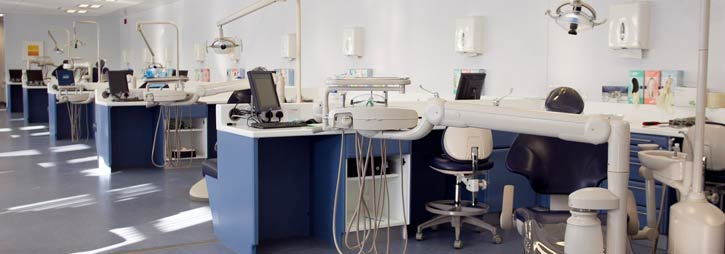
\includegraphics[width=6cm]{images/OrthoClinic}
\end{textblock*}
\begin{columns}[b]
\begin{column}{0.5\textwidth}
\begin{itemize}
\item Real-World Problem
\begin{itemize}
\item Change time table during period of teaching capacity increase
\item Previous schedule no longer feasible
\item Multiple courses share same lab space (dental chairs) at the same time
\item Hard capacity limits on available resources and time slots
\end{itemize}
\item Status
\begin{itemize}
\item Used by dental school during transition period
\item Paper in IAAI 2013, AI Mag 2014
\end{itemize}
\end{itemize}
\end{column}
\begin{column}{0.5\textwidth}
\begin{itemize}
\item Research Challenges
\begin{itemize}
\item Very different from standard timetabling problem
\item Hard/soft capacity constraints
\item Tool cleaning setup time constraints
\end{itemize}
\item Solution Approach
\begin{itemize}
\item Optimization
\item Flexible prioritization of constraints
\end{itemize}
\end{itemize}
\end{column}
\end{columns}
\end{frame}

\begin{frame}
\frametitle{Irish Naval Service Yearly Rostering}
\begin{textblock*}{4cm}(9cm,-1cm)
%
\includegraphics[width=2.5cm]{images/Irish_Naval_Service}
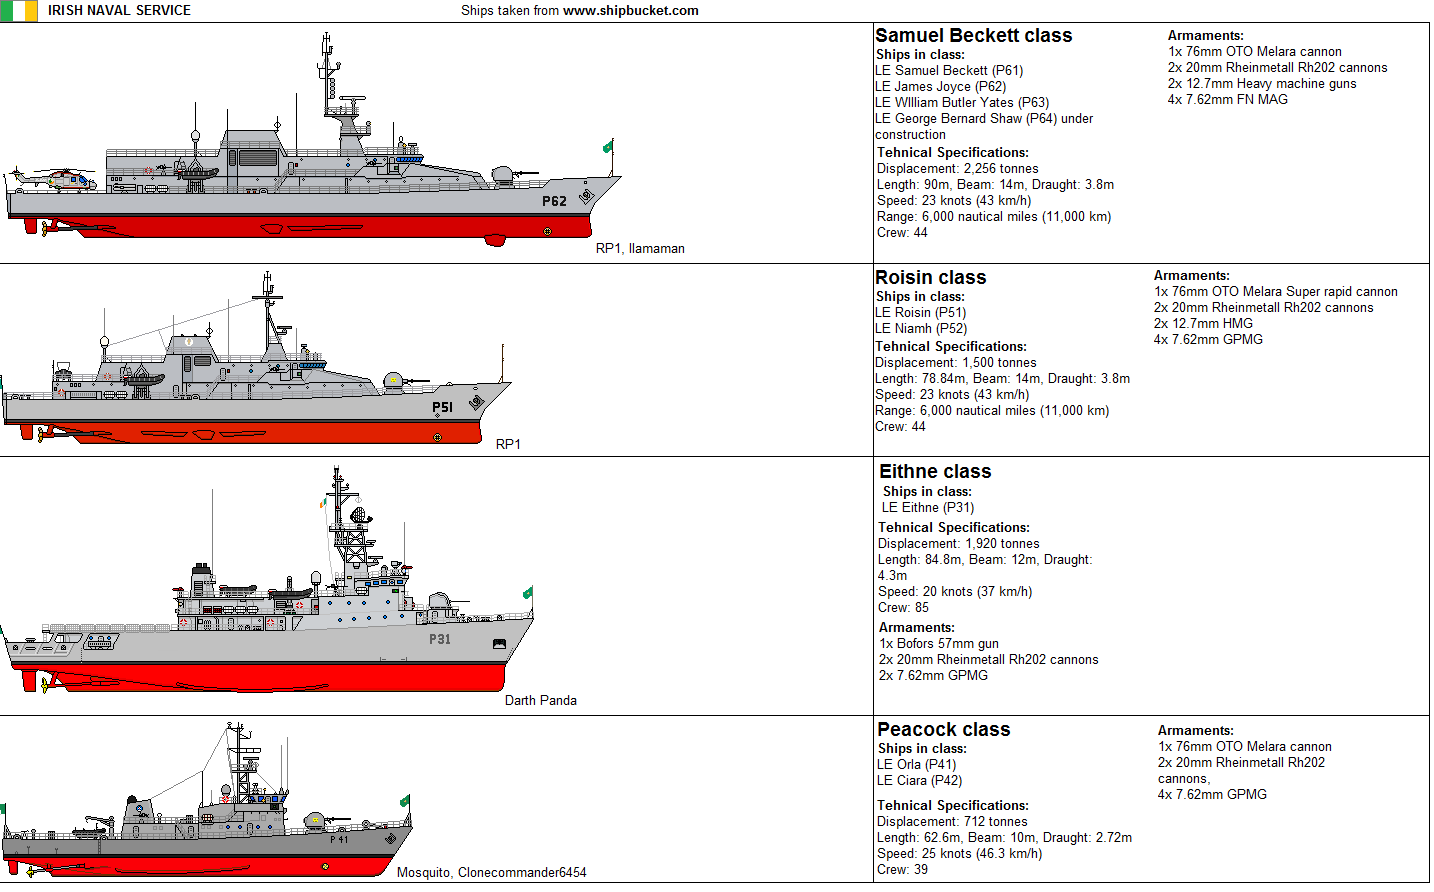
\includegraphics[width=4cm]{images/irish_naval_service_by_zagoreni010_dbaxsq7}
\end{textblock*}
\vspace{1cm}

\begin{columns}[b]
\begin{column}{0.5\textwidth}
\begin{itemize}
\item Real-World Problem
\begin{itemize}
\item Decide which ships are performing which type of duty over the year
\item Budget limitations on total time at sea
\item Fair share of work across fleet
\item Fixed maintenance periods for certain ships
\item Special events (flotilla exercises, detached duty) 
\end{itemize}
\item Status
\begin{itemize}
\item Prototype results produced for service
\end{itemize}
\end{itemize}
\end{column}
\begin{column}{0.5\textwidth}
\begin{itemize}
\item Research Challenges
\begin{itemize}
\item Finding the best tool and model for problem
\item Balanced assignment under budget constraints
\item Provide consistent force levels over whole year
\item Fair assignment of work/rest days across fleet
\end{itemize}
\item Solution Approach
\begin{itemize}
\item Optimization
\end{itemize}
\end{itemize}
\end{column}
\end{columns}
\end{frame}

\begin{frame}
\frametitle{Data Centre Load Consolidation}
\begin{textblock*}{7cm}(8cm,-1cm)
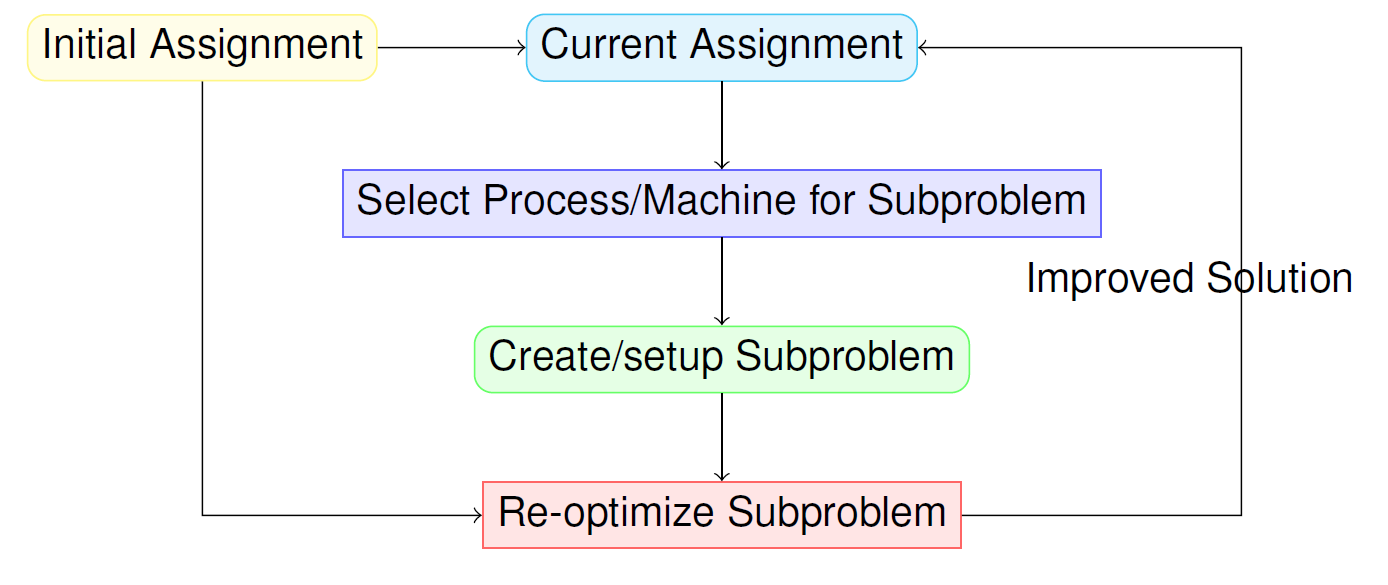
\includegraphics[width=7cm]{images/lnsdesign}
\end{textblock*}
\vspace{1cm}
\begin{columns}[b]
\begin{column}{0.5\textwidth}
\begin{itemize}
\item Real-World Problem
\begin{itemize}
\item Move virtual machines between servers in a data centre
\item Balance/concentrate workload on multiple resource types
\item Extend to multiple data centres across world 
\end{itemize}
\item Status
\begin{itemize}
\item 2nd place in Google Roadef/Euro Challenge 2012
\item Multiple papers
\end{itemize}
\end{itemize}
\end{column}
\begin{column}{0.5\textwidth}
\begin{itemize}
\item Research Challenges
\begin{itemize}
\item Reassignment problem
\item Multi-bin packing constraints
\item Large neighbourhood search to deal with problem size 
\end{itemize}
\item Solution Approach
\begin{itemize}
\item Optimization
\item New tools/propagators
\end{itemize}
\end{itemize}
\end{column}
\end{columns}
\end{frame}

\begin{frame}
\frametitle{Scheduling with Time Variable Energy Prices}
\begin{textblock*}{3cm}(11cm,-1cm)
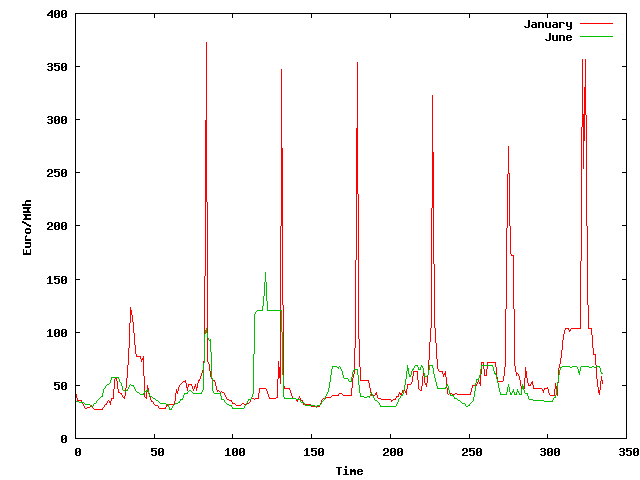
\includegraphics[width=3cm]{images/price}
\end{textblock*}
\vspace{0.8cm}
\begin{columns}[b]
\begin{column}{0.5\textwidth}
\begin{itemize}
\item Real-World Problem
\begin{itemize}
\item How do time-variable electricity prices affect scheduling of use
\item Uncertainty of prices, sudden peak prices common in Ireland
\item In most cases, we have to commit to production before price is known
\item Deal with risk/possible rewards
\end{itemize}
\item Status
\begin{itemize}
\item Multiple papers 
\item Continued work on price prediction with industry
\end{itemize}
\end{itemize}
\end{column}
\begin{column}{0.5\textwidth}
\begin{itemize}
\item Research Challenges
\begin{itemize}
\item Can we use time variable electricity prices to our advantage?
\item Which properties should a price prediction model have to help with scheduling?
\item Can we tune price prediction for the use case it is intended for?
\end{itemize}
\item Solution Approach
\begin{itemize}
\item Machine Learning
\item Optimization
\end{itemize}
\end{itemize}
\end{column}
\end{columns}
\end{frame}

\begin{frame}
\frametitle{Characterizing EDF Power Plants}
\begin{textblock*}{3cm}(10cm,-1cm)
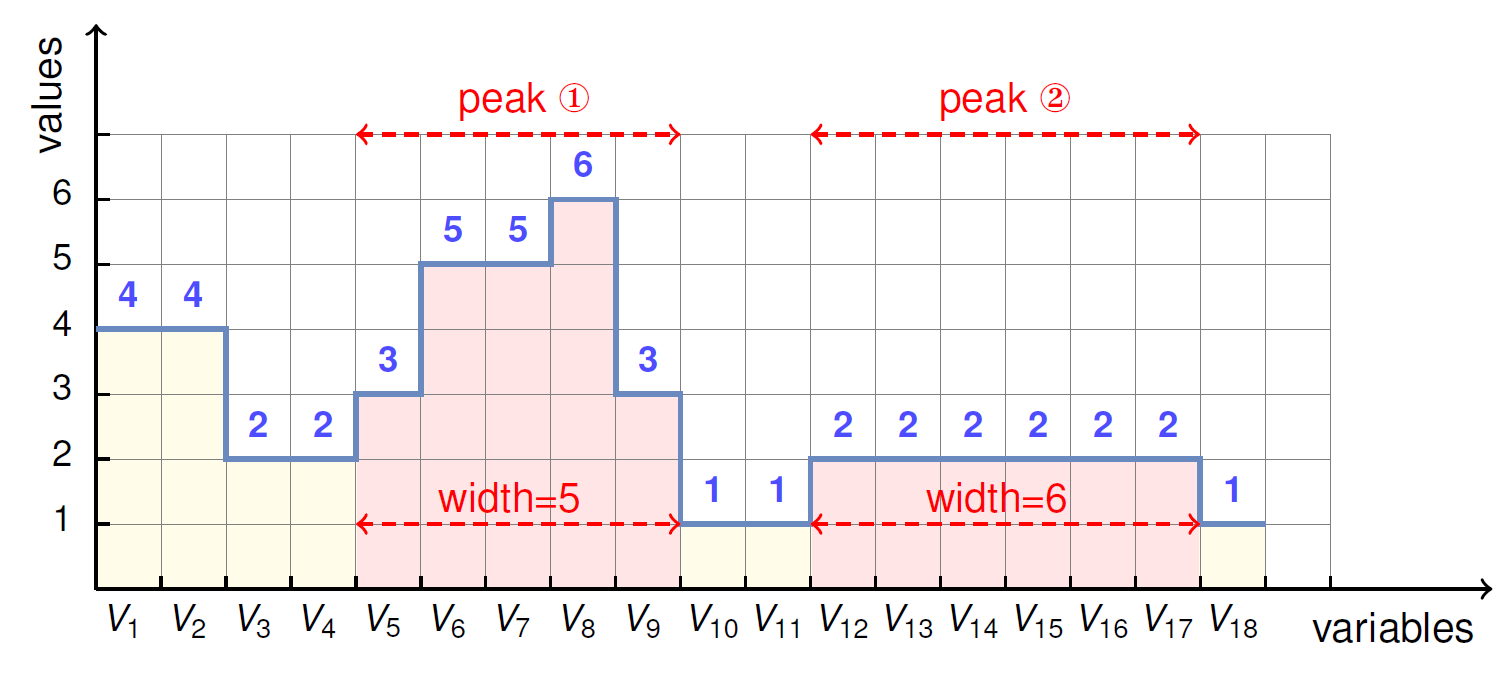
\includegraphics[width=3cm]{images/minwidthpeak}
\end{textblock*}

\begin{columns}[b]
\begin{column}{0.5\textwidth}
\begin{itemize}
\item Real-World Problem
\begin{itemize}
\item Unit Commitment Model for electricity supply
\item Decide which units to run when to satisfy demand/minimize cost
\item Change of production for different units is limited over time
\item Very error-prone integration into global model
\end{itemize}
\item Status
\begin{itemize}
\item Joint work with IMT-Atlantique, EDF Research
\item Series of papers on time-series constraints, Volume II of Global Constraint Catalog
\end{itemize}
\end{itemize}
\end{column}
\begin{column}{0.5\textwidth}
\begin{itemize}
\item Research Challenges
\begin{itemize}
\item Can we characterize the production limits of power plants as time-series constraints?
\item Learn constraints from historical data (planned/actual)
\item Create model of individual plants to describe their capabilities
\item Find redundant constraints to overcome limits of propagation  
%\item Integrate into MIP unit commitment model
\end{itemize}
\item Solution Approach
\begin{itemize}
\item Machine Learning
\item Automata constraints
\item Generated code for propagators
\end{itemize}
\end{itemize}
\end{column}
\end{columns}
\end{frame}

\begin{frame}
\frametitle{Optical Network Design}
\begin{textblock*}{6cm}(8cm,-1cm)
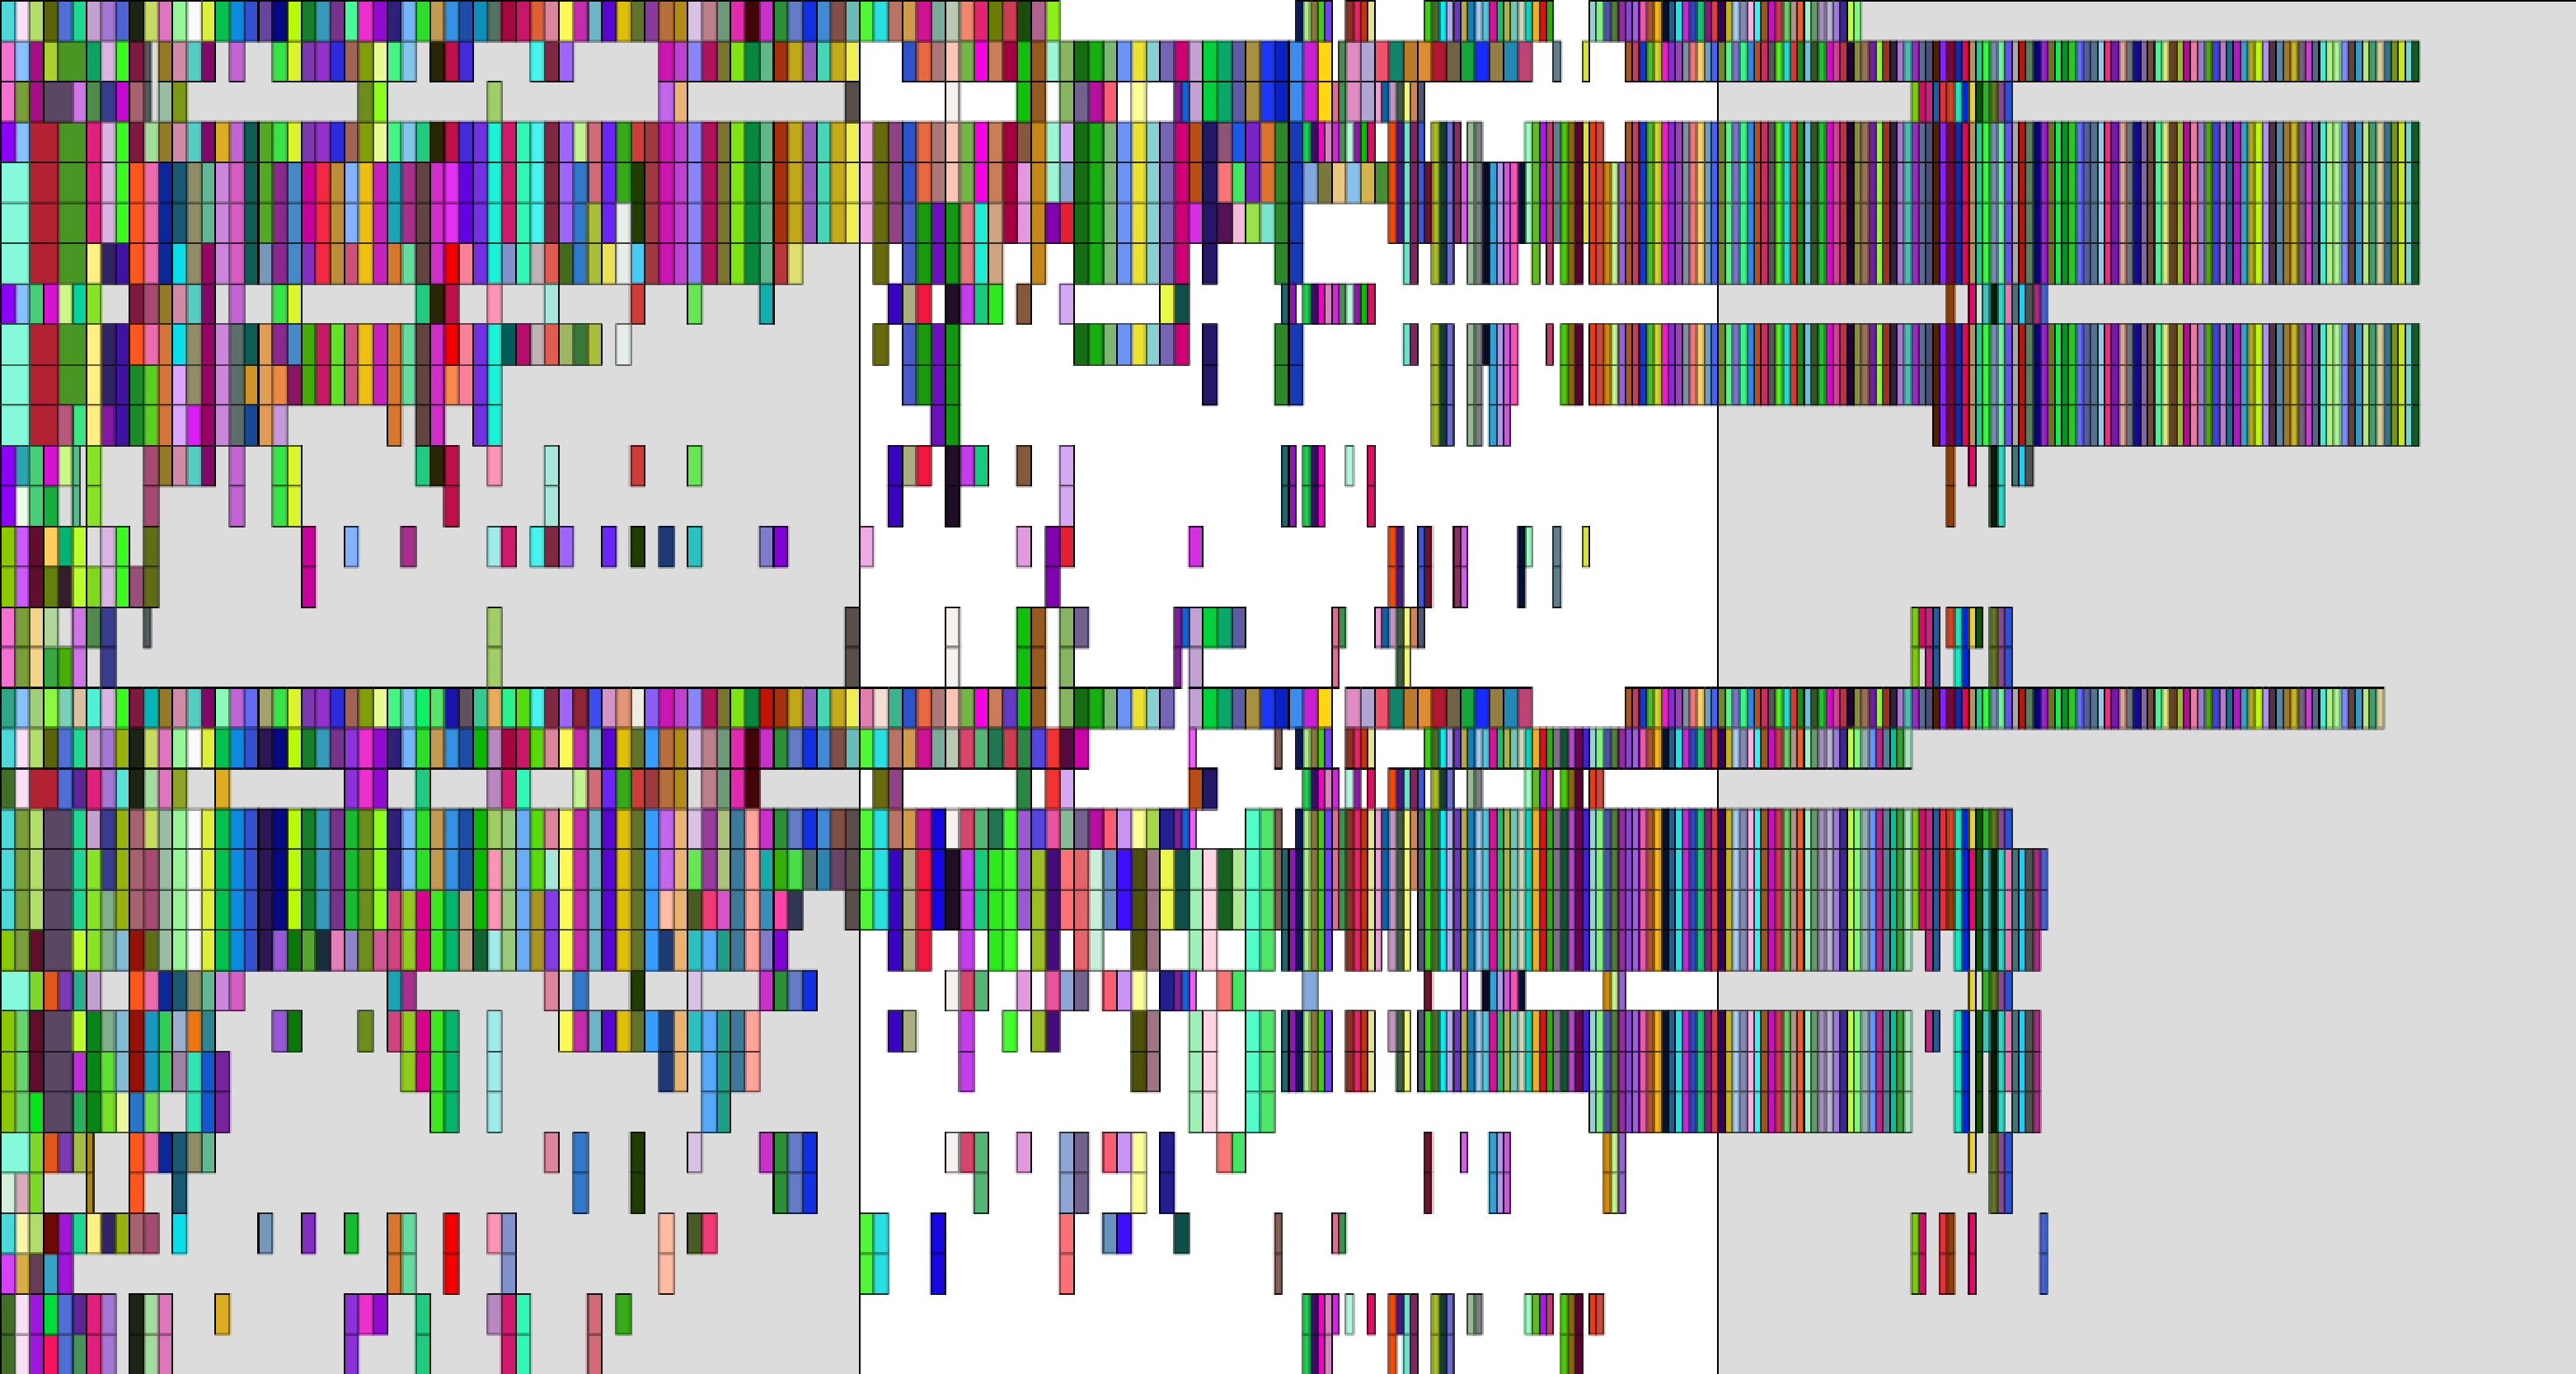
\includegraphics[width=6cm]{images/Ireland18}
\end{textblock*}
\vspace{1cm}
\begin{columns}[b]
\begin{column}{0.5\textwidth}
\begin{itemize}
\item Real-World Problem
\begin{itemize}
\item Core optical network design 
\item Different from traditional IP network design
\item Define paths from source to sink
\item Use multiple frequency (light) bands over same fibre
\end{itemize}
\item Status
\begin{itemize}
\item Paper ICTAI 2014
\end{itemize}
\end{itemize}
\end{column}
\begin{column}{0.5\textwidth}
\begin{itemize}
\item Research Challenges
\begin{itemize}
\item Modelling Choices
\item Amount of propagation achieved
\item Scalability of methods
\end{itemize}
\item Solution Approach
\begin{itemize}
\item Global Constraints
\end{itemize}
\end{itemize}
\end{column}
\end{columns}
\end{frame}

\begin{frame}
\frametitle{Supplier Selection Problem}
\begin{textblock*}{9cm}(6cm,-1cm)
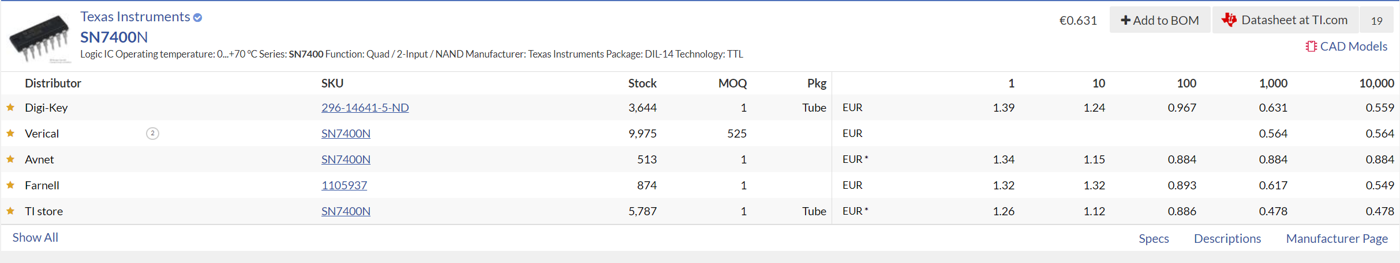
\includegraphics[width=9cm]{images/sn7400}
\end{textblock*}
\vspace{1cm}
\begin{columns}[b]
\begin{column}{0.5\textwidth}
\begin{itemize}
\item Real-World Problem
\begin{itemize}
\item Which suppliers to select to provide list of components
\item Limit number of suppliers by ordering multiple items from same supplier
\item Price/lead time/quality of service are competing objectives
\end{itemize}
\item Status
\begin{itemize}
\item Work with industry partner
\item Paper in Annals of Operations Research
\end{itemize}
\end{itemize}
\end{column}
\begin{column}{0.5\textwidth}
\begin{itemize}
\item Research Challenges
\begin{itemize}
\item How do we learn which choices are preferred
\item Difficult to assign fixed weights to different aspects of solution quality
\item Iterative, interactive learning of preferences
\end{itemize}
\item Solution Approach
\begin{itemize}
\item Preference Learning
\item Optimization
\end{itemize}
\end{itemize}
\end{column}
\end{columns}
\end{frame}

\begin{frame}
\frametitle{Optimizing UCC's CHP Plant Operation}
\begin{textblock*}{3.5cm}(10cm,-1cm)
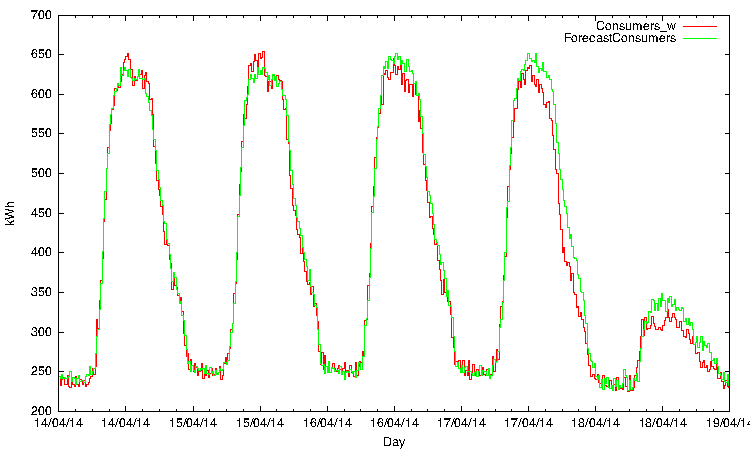
\includegraphics[width=3.5cm]{images/campusdemand}
\end{textblock*}
\vspace{0.5cm}
\begin{columns}[b]
\begin{column}{0.5\textwidth}
\begin{itemize}
\item Real-World Problem
\begin{itemize}
\item When to run UCC's CHP plant to create electricity/heat on-site
\item Needs demand forecast for heat and electricity
\item Uncertain Real-time grid electricity price
\item Heat and electricity demand of campus not in sync
\end{itemize}
\item Status
\begin{itemize}
\item Tested for several weeks with operator of plant
\item Part of EU Campus21 project
\end{itemize}
\end{itemize}
\end{column}
\begin{column}{0.5\textwidth}
\begin{itemize}
\item Research Challenges
\begin{itemize}
\item Heat and Electricity Demand prediction for campus
\item Price prediction for real-time grid price
\item Integration of plant operational constraints
\item Wider impact of heating strategy on campus 
\end{itemize}
\item Solution Approach
\begin{itemize}
\item Machine Learning
\item Optimization
\end{itemize}
\end{itemize}
\end{column}
\end{columns}
\end{frame}

\begin{frame}
\frametitle{CP Conference Paper Assignment Tool}
\begin{textblock*}{4cm}(10cm,-1cm)

\includegraphics[width=4cm]{images/cp2020logo}
\end{textblock*}
\begin{textblock*}{3cm}(10cm,0.5cm)

\includegraphics[width=3cm]{images/cp2021logo}
\end{textblock*}
\begin{columns}[b]
\begin{column}{0.5\textwidth}
\begin{itemize}
\item Real-World Problem
\begin{itemize}
\item Which reviewers to assign to papers 
\item Consider bids by reviewers, avoid assigning unwanted papers
\item Deal with reviewers shared between multiple tracks 
\item Balance assignment between reviewers
\item Allow pre-assignment, specific capacity constraints
\end{itemize}
\item Status
\begin{itemize}
\item Joint work with Data61, INRA
\item Used in 2020, 2021
\item Paper at ModRef 2020
\end{itemize}
\end{itemize}
\end{column}
\begin{column}{0.5\textwidth}
\begin{itemize}
\item Research Challenges
\begin{itemize}
\item Fair treatment of papers and reviewers
\item Finding mechanisms to allow Program Chair to control process
\item Not a black-box assignment
\item Integration with easychair
\end{itemize}
\item Solution Approach
\begin{itemize}
\item Optimization
\end{itemize}
\end{itemize}
\end{column}
\end{columns}
\end{frame}

